\section{General GPU Architecture}
\label{sec:gpu}

The \textbf{General-purpose computation on graphics processing units (GPGPU)} is a microprocesser that performs computation traditionally handled by the CPU.
In our project we only work with CUDA-enabled devices, but we assume that the features of CUDA-enabled devices are equivalent to thoese of GPGPUs for the ease of notation.
The GPGPU consists of a large amount of simple and economical processing units that individually are weaker than the CPU, but combined possess upto several magnitudes of larger throughput.
The GPGPU is attached to the CPU, such that the CPU utilizes the GPGPU, to accelerate computation that the GPGPU is more suitable at handling, e.g. processes that are parallel.

\begin{figure}[htb]
  \centering
  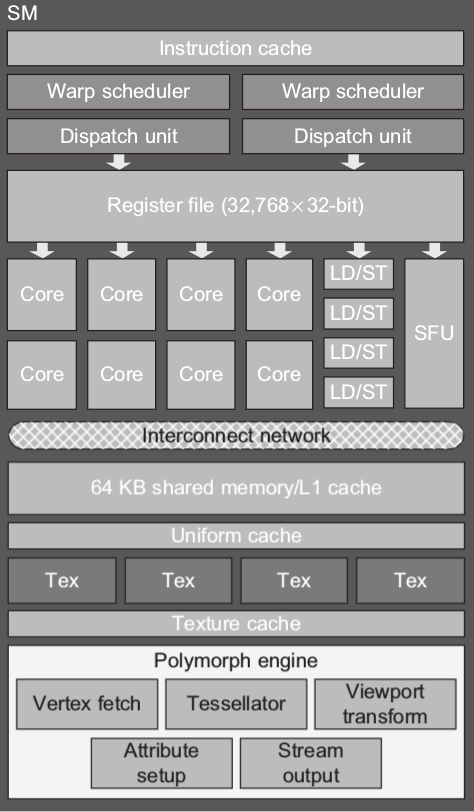
\includegraphics[width=.5\textwidth]{graphics/images/cropped-cuda-sm.png}
  \caption{Example of a Streaming Multiprocessor for reference~\cite{farber2011cuda}}
  \label{fig:sm example}
\end{figure}

The GPGPU's architecture is based on a parallel scheme, which has promoted an architecture of independance among processing cores on the GPGPU.
The basic building block of this architecture is the streaming multiprocessor (SM) shown in \cref{fig:sm example}, which is independently responsible for its own resources, cores, and memory.
By making each SM independent, memory access and computation are performed faster as the memory is placed physically closer to the cores.
The cores on each SM are Single Instruction, Multiple Data (SIMD) ALUs.
As the cores are constrained to run the same piece of code, though with different data, the software paradigm of ``kernels'' has developed.
A kernel is a describtion of a set of instruction that all cores across all SMs performs independantly of one another.
The work given to the GPU is distributed to the SMs by the Giga-Thread global scheduler.
The Giga-thread scheduler holds metainformation on the SMs, which allows it to optimize workloads across the GPGPU's independent processors.
The SMs receive instructions from the scheduler in a cache schedules the work for execution on the cores in the SM.
We will go more into depth regarding the specifics on scheduling of independant processes in \cref{chap:software}.

At runtime, every independant process has access to its own registers called local memory.
Each SM has shared memory for high-speed data sharing between threads in a block called shared memory.
To supply the SMs with data the GPGPU contains a larger amount of global data available to all SMs.

Furthermore, a SM has load/store (LD/ST) units and Special Function Units (SFU).
LD/STs calculates source and destination addresses and loads/store data as needed.
SFUs execute special functions, e.g. sin, sqrt, etc.
Compared to the SIMD cores, the SFUs are designed specifically to perform their designated functions whereas the SIMD cores are general purpose cores~\cite{fermi2009nvidia}.

% good warp answers:  http://stackoverflow.com/questions/11816786/why-bother-to-know-about-cuda-warps
%                     http://stackoverflow.com/questions/10460742/how-do-cuda-blocks-warps-threads-map-onto-cuda-cores

\subsection{Hardware Specific Numbers}
\label{sec:hardware specific numbers}
Using CUDA functionality we are able to extract hardware specific numbers from the GPGPU.
We we use the hardware specification in \cref{optimization} as to how we utilize the given architecture to optimize our kernel to the hardware.

Throughout this report, we will be using the Tesla K40 GPU~\cite{teslak402013nvidia}.
For future reference \cref{tab:tesla k40 specs} presents the specifications for our GPU device.
In \cref{ap:tesla k40 specifications} we desribe which commands were used to find the specifications for our device.
\todo{is L1 cache used for shared memory?}

\begin{table}[htb]
  \centering
  \begin{tabular}{l r}
    \toprule
    item                        & limit \\
    \midrule
    warp size                   & \SI{32}{} \\
    max threads / block         & \SI{1024}{} \\
    total cores                 & \SI{2880}{} \\
    registers / block           & \SI{65536}{} \\
    constant memory             & \SI{65536}{B} \\
    L1 cache / block            & \SI{49152}{B}  \\
    L2 cache / core             & \SI{1572864}{B}  \\
    global memory               & \SI{12079136768}{B} \\
    \bottomrule
  \end{tabular}
  \caption{Tesla K40 GPU's specifications}
  \label{tab:tesla k40 specs}
\end{table}

Furthermore, the maximum dimension of grids and blocks are presented in \cref{tab:tesla k40 grid and block}.

\begin{table}[htb]
  \centering
  \begin{tabular}{r r r r}
    \toprule
    item & x & y & z \\
    \midrule
    block size & \SI{1024}{} & \SI{1024}{} & \SI{64}{} \\
    grid size  & \SI{2147483647}{} & \SI{65535}{} & \SI{65535}{} \\
    \bottomrule
  \end{tabular}
  \caption{Tesla K40 GPU's block and grid sizes}
  \label{tab:tesla k40 grid and block}
\end{table}
